% ***********************************************************
% ******************* PHYSICS HEADER ************************
% ***********************************************************
% Version 2
\documentclass[11pt]{article} 
\usepackage{amsmath} % AMS Math Package
\usepackage{amsthm} % Theorem Formatting
\usepackage{amssymb}	% Math symbols such as \mathbb
\usepackage{graphicx} % Allows for eps images
\usepackage{multicol} % Allows for multiple columns
\usepackage[dvips]{geometry}
 % Sets margins and page size
\pagestyle{empty} % Removes page numbers
\makeatletter % Need for anything that contains an @ command 
\renewcommand{\maketitle} % Redefine maketitle to conserve space
{ \begingroup \vskip 10pt \begin{center} \large {\bf \@title}
	\vskip 10pt \large \@author \hskip 20pt \@date \end{center}
  \vskip 10pt \endgroup \setcounter{footnote}{0} }
\makeatother % End of region containing @ commands
\renewcommand{\labelenumi}{(\alph{enumi})} % Use letters for enumerate
% \DeclareMathOperator{\Sample}{Sample}
\let\vaccent=\v % rename builtin command \v{} to \vaccent{}
\renewcommand{\v}[1]{\ensuremath{\mathbf{#1}}} % for vectors
\newcommand{\gv}[1]{\ensuremath{\mbox{\boldmath$ #1 $}}} 
% for vectors of Greek letters
\newcommand{\uv}[1]{\ensuremath{\mathbf{\hat{#1}}}} % for unit vector
\newcommand{\abs}[1]{\left| #1 \right|} % for absolute value
\newcommand{\avg}[1]{\left< #1 \right>} % for average
\let\underdot=\d % rename builtin command \d{} to \underdot{}
\renewcommand{\d}[2]{\frac{d #1}{d #2}} % for derivatives
\newcommand{\dd}[2]{\frac{d^2 #1}{d #2^2}} % for double derivatives
\newcommand{\pd}[2]{\frac{\partial #1}{\partial #2}} 
% for partial derivatives
\newcommand{\pdd}[2]{\frac{\partial^2 #1}{\partial #2^2}} 
% for double partial derivatives
\newcommand{\pdc}[3]{\left( \frac{\partial #1}{\partial #2}
 \right)_{#3}} % for thermodynamic partial derivatives
\newcommand{\ket}[1]{\left| #1 \right>} % for Dirac bras
\newcommand{\bra}[1]{\left< #1 \right|} % for Dirac kets
\newcommand{\braket}[2]{\left< #1 \vphantom{#2} \right|
 \left. #2 \vphantom{#1} \right>} % for Dirac brackets
\newcommand{\matrixel}[3]{\left< #1 \vphantom{#2#3} \right|
 #2 \left| #3 \vphantom{#1#2} \right>} % for Dirac matrix elements
\newcommand{\grad}[1]{\gv{\nabla} #1} % for gradient
\let\divsymb=\div % rename builtin command \div to \divsymb
\renewcommand{\div}[1]{\gv{\nabla} \cdot #1} % for divergence
\newcommand{\curl}[1]{\gv{\nabla} \times #1} % for curl
\let\baraccent=\= % rename builtin command \= to \baraccent
\renewcommand{\=}[1]{\stackrel{#1}{=}} % for putting numbers above =
\newtheorem{prop}{Proposition}
\newtheorem{thm}{Theorem}[section]
\newtheorem{lem}[thm]{Lemma}
\theoremstyle{definition}
\newtheorem{dfn}{Definition}
\theoremstyle{remark}
\newtheorem*{rmk}{Remark}

% ***********************************************************
% ********************** END HEADER *************************
% ***********************************************************

%%% Local Variables:
%%% mode: latex
%%% TeX-Master: notes
%%% End:

\usepackage[utf8]{inputenc}
\usepackage{amsmath}
\usepackage{amssymb}
\usepackage{amsfonts}
\usepackage{amssymb}
\usepackage{float}
\usepackage{indentfirst}
\usepackage{vmargin}
\usepackage{indentfirst}
\usepackage{titling}
\usepackage{color} 
\usepackage{siunitx}
\usepackage{xspace}
\usepackage{graphicx}
\usepackage{enumitem}
\usepackage[backend=biber,backref=true,style=unsrt,
style=numeric-comp,block=ragged,firstinits=true]{biblatex}
\addbibresource{ref-notes.bib}
\bibliography{ref-notes}
\graphicspath{{TD6/}}

\newcommand{\mastersig}{\ensuremath{\Im{\widehat{\Sigma}^{A,B}(k,E)}}\xspace}
\newcommand{\chiqw}{\ensuremath{\Im{\chi}(q,\omega)}\xspace}

\providecommand{\norm}[1]{\lVert#1\rVert}

\newcommand{\subtitle}[1]{%
  \posttitle{%
    \par\end{center}
    \begin{center}\large#1\end{center}
    \vskip0.5em}%
}


\title{Condensed Matter II}
\subtitle{Problem set \#4}
%\author{}
\date{Spring 2014}

\begin{document}

\maketitle

\setlength{\unitlength}{1cm}
%\advance\textwidth by 3cm
%\advance\hoffset by -1.5cm 
\advance\textheight by 1cm
\advance\voffset by -1.5cm
\setmarginsrb{3cm}{0.5cm}{1.5cm}{1cm}{1cm}{1cm}{1cm}{1cm}
%\setlength{\parindent}{0cm}%

\pagestyle{plain}

\section{Free electrons in Na}

\begin{figure}[h]
  \centering
  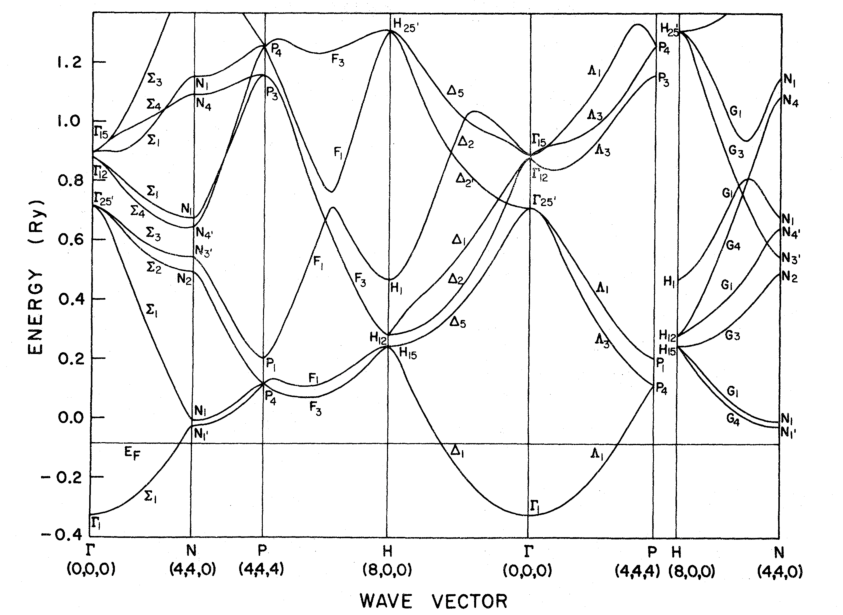
\includegraphics[width=14cm]{NA_bands.pdf}
  \caption{Energy bands in sodium along symmetry directions. Chang
    and Callaway, PRB 11, 1324 (1975) \label{fig:bands}}
\end{figure}

\subsection{Qualitative study}

\begin{enumerate}[label=(\roman*)]
\item With the help of the computed band structure of Na in Fig.~\ref{fig:bands}, suggest what the structure of the empty BCC lattice must look
  like (assuming isotropic effective mass $m_0$).
\item How high above the bottom of the conduction band is the Fermi
  energy located in this model?
\item Justify that Na may be considered ``the simplest of the simple metals''.
\end{enumerate}

\subsection{Quantitative study}

\begin{enumerate}[label=(\roman*)]
\item Use Bloch's theorem to give the general expression of the energy
  $E_l(k)$ in a general 3D crystal, where $l \equiv (l_1,l_2,l_3)$ is
  the band index, and $k$ is a wave vector.
\item A schematic of the Brillouin zone of the
  BCC lattice is provided in Fig.~\ref{fig:lattice}. Use the previously
  obtained result, and derive the expression of the energy levels at
  the special points $\Gamma$, $H$, $P$, and  $N$ in the empty BCC lattice.
\item Use you favorite computation/programming/plotting tool to
  draw the approximate shape of the band structure of the empty BCC
  lattice, which should follow the conclusions drawn from the
  qualitative study.
\end{enumerate}

\begin{figure}[h]
  \centering
  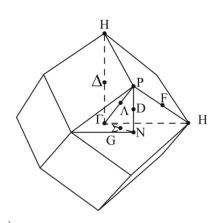
\includegraphics[width=10cm]{BCC_lattice.pdf}
  \caption{Brillouin zone for the bocy-centered cubic
    lattice. M. Dresselhaus, Group theory - Application to the
    Physics of Condensed Matter, Fig. C.5.b, p 511. \label{fig:lattice}}
\end{figure}

%\section

\end{document}